\chapter{Geometry and conventions}
\label{ch:geometry}

\section{Frames of reference and units}

Two frames are used.
\begin{description}
  \item[Lab frame.] The $z$ axis is the direction of the incident beam, $x$ is horizontal
        and $y$ is vertical. The origin is the centre of rotation of the instrument, that is, the centre of the circle
        on which the detector moves. All the data given by the user (beam, detector angle, directions) are in this frame.
  \item[Sample frame.] A frame attached to the sample, in which its geometry is simplest. For a slab,
        or a disc, $z'$ is the normal of the layers; for a vertical cylinder and for a sphere it coincides with the lab frame. The
        samples convert between the two with \code{to_sample_frame} and \code{to_lab_frame}.
\end{description}
All lengths are in millimetres; linear attenuation coefficients are in mm$^{-1}$.

\section{The instrument}

The detector of a two-axis instrument moves on a circle in the horizontal plane $y=0$, centred on the sample
(Figure~\ref{fig:instrument}). The scattering angle $\twotheta$ is the angle between the direction of the
scattered particle and the direction of the incident beam ($+z$). It is measured from $+z$ towards $+x$, and
runs from $0^\circ$ (forward) to $180^\circ$ (backward).

\begin{figure}[ht]
  \centering
  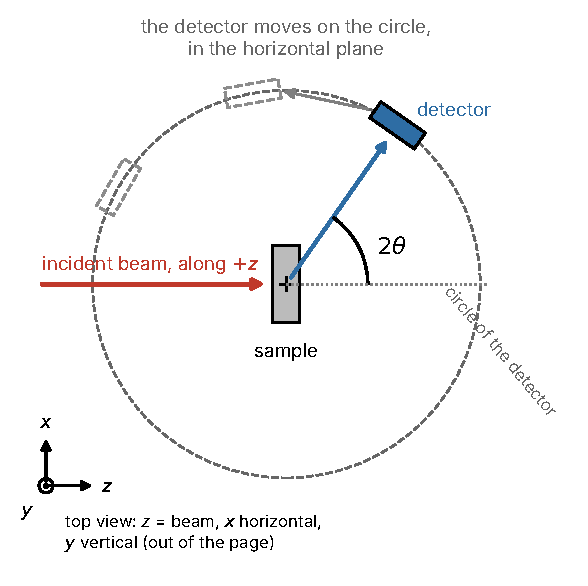
\includegraphics[width=0.78\textwidth]{fig_instrument}
  \caption{Top view of the instrument. The beam travels along $+z$ and hits the sample at the centre of the circle
  of the detector; the angle $\twotheta$ is measured between the incident direction and the direction of the detector.}
  \label{fig:instrument}
\end{figure}

A direction in space is given by two angles, the polar angle $\twotheta$ (from the beam) and the azimuth
$\varphi$ (around the beam, from $+x$ towards $+y$):
\begin{equation}
  \hat{d} = (\sin\twotheta\cos\varphi,\; \sin\twotheta\sin\varphi,\; \cos\twotheta).
\end{equation}
A detector in the horizontal plane has $\varphi=0$ (towards $+x$) or $\varphi=180^\circ$ (towards $-x$). This is
what the function \code{scattered_direction(two_theta_deg, phi_deg=0.0)} returns.

\section{The beam}

The beam is a rectangle of width $w_b$ (along $x$) and height $h_b$ (along $y$), centred on the beam axis and
perpendicular to $z$. Its intensity is described by two independent profiles, $H(x)$ and $V(y)$ (Chapter~\ref{ch:beam}).
A particle is identified by the point $(x,y)$ where it starts, in the plane perpendicular to the beam that contains
the origin.

\section{Vertical position of the sample}

Slab and cylinder have a height and a bottom, $y_\mathrm{bottom}$ (argument \code{y_bottom}). By default the sample is
centred on the beam: $y_\mathrm{bottom}=-\text{height}/2$, and it extends to $y_\mathrm{top}=y_\mathrm{bottom}+\text{height}$.
The disc and the sphere are always centred on the beam: they go from $-R$ to $+R$. In every geometry the material of a layer can occupy
only a band of heights, from its own bottom to its own top (Chapter~\ref{ch:partial}).

\section{The slab geometry}

The slab is a stack of flat layers (Figure~\ref{fig:slab}). Its section is a rectangle of width $w$ (horizontal)
and height $h$ (vertical), centred on the beam horizontally and, by default, vertically. The layers are given \emph{from the front face to the back}, each one with
its thickness along the normal $z'$.

The orientation is set by the \textbf{plane angle} $\alpha$ (\code{plane_angle_deg}): the angle between the incident beam
and the plane of the sample.
\begin{itemize}
  \item $\alpha=90^\circ$ (default): the plane is perpendicular to the beam (normal incidence); the sample frame and the lab
        frame coincide.
  \item $\alpha<90^\circ$: the sample is rotated around the vertical axis and its normal is tilted towards $+x$ by
        $\omega = 90^\circ-\alpha$. For $\alpha>90^\circ$ it is tilted towards $-x$.
  \item Values of $\alpha$ very close to $0^\circ$ or $180^\circ$ (beam parallel to the plane) are not allowed.
\end{itemize}
The axis of rotation is the vertical line through the centre of the front face, which lies on the beam axis.

\begin{figure}[ht]
  \centering
  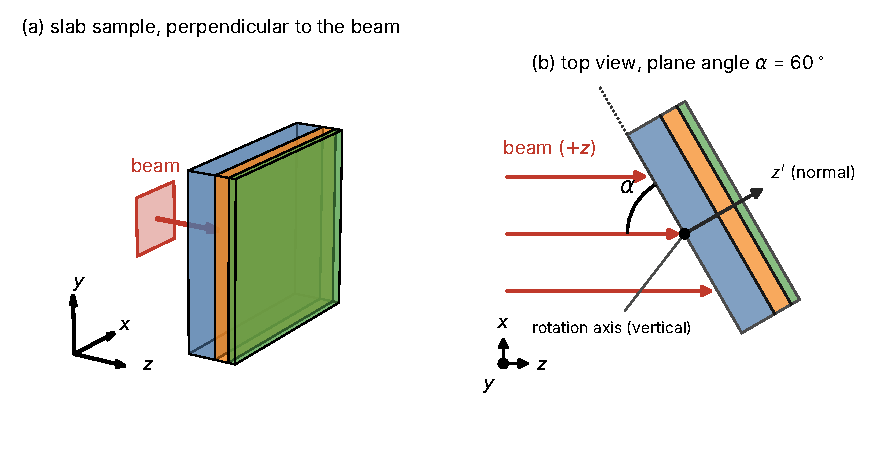
\includegraphics[width=\textwidth]{fig_slab_geometry}
  \caption{Slab geometry. (a)~Perspective view of a three-layer slab perpendicular to the beam; the red rectangle is the beam.
  (b)~Top view of the same sample rotated so that the angle between the beam and the plane of the sample is
  $\alpha=60^\circ$; $z'$ is the normal of the layers.}
  \label{fig:slab}
\end{figure}

\section{The disc geometry}

The disc (version 2.3) is a slab with a circular section: layers stacked along the normal $z'$, all with the same diameter
$D$, centred on the beam axis, and rotated around the vertical axis with the same plane angle $\alpha$ as the slab. It is
described in Chapter~\ref{ch:disc} (Figure~\ref{fig:disc}).

\section{The cylindrical geometry}

The sample is a set of concentric cylinders whose common axis is vertical and passes through the centre of the
instrument (Figure~\ref{fig:cylinder}). All the cylinders have the same height. The layers are given \textbf{from the
inner one outwards}:
\begin{itemize}
  \item the first layer is a full cylinder and its ``thickness'' is its \textbf{diameter}, so its radius is $r_1 = t_1/2$;
  \item the following layers are annuli and their thickness is the radial thickness: $r_k = r_{k-1} + t_k$.
\end{itemize}
For instance, the thicknesses $(6.0,\,1.0,\,0.5)$~mm give the radii $(3.0,\,4.0,\,4.5)$~mm and an outer diameter of 9~mm.
Because the cylinder is symmetric around its axis there is no orientation parameter. Particles can leave the sample through
the side surface and through the flat ends. All the cylinders start at the same bottom; each of them can be filled only up to
a given level (Chapter~\ref{ch:partial}).

\begin{figure}[ht]
  \centering
  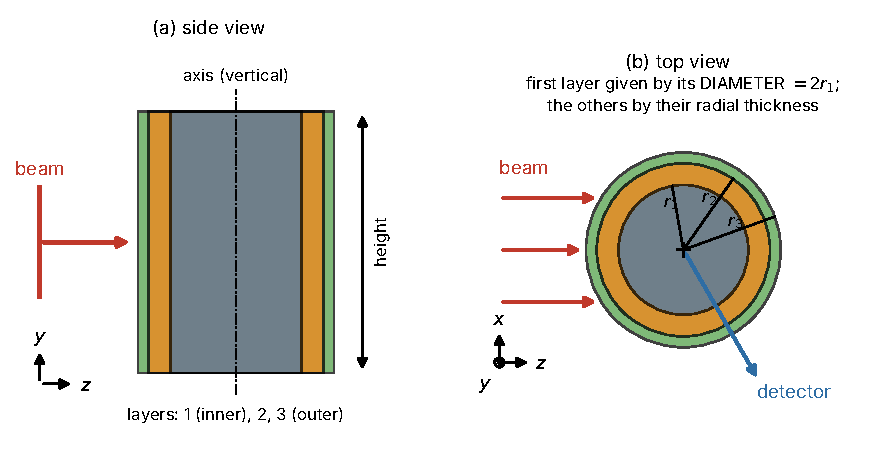
\includegraphics[width=\textwidth]{fig_cylinder_geometry}
  \caption{Cylindrical geometry. (a)~Side view: concentric cylinders of the same height, vertical axis. (b)~Top view:
  the radii $r_1<r_2<r_3$; the thickness of the first layer is its diameter $2r_1$.}
  \label{fig:cylinder}
\end{figure}

\section{The spherical geometry}

The sphere (version 2.4) is a set of concentric spheres centred on the beam axis, at the centre of the instrument. As for the
cylinder, the layers are given from the inner one outwards: the thickness of the first is its diameter, the others are radial
thicknesses. There is no orientation parameter. It is described in Chapter~\ref{ch:sphere} (Figure~\ref{fig:sphere}).

\section{Example trajectories}

Figure~\ref{fig:traj} shows, in top view, a few particles in both geometries: they enter along $+z$, interact at the
points marked with the colour of the layer in which they happen, and are then followed in the direction of a detector
at $\twotheta=100^\circ$ until they leave the sample. These are the paths that the package computes for thousands of
particles at once.

\begin{figure}[ht]
  \centering
  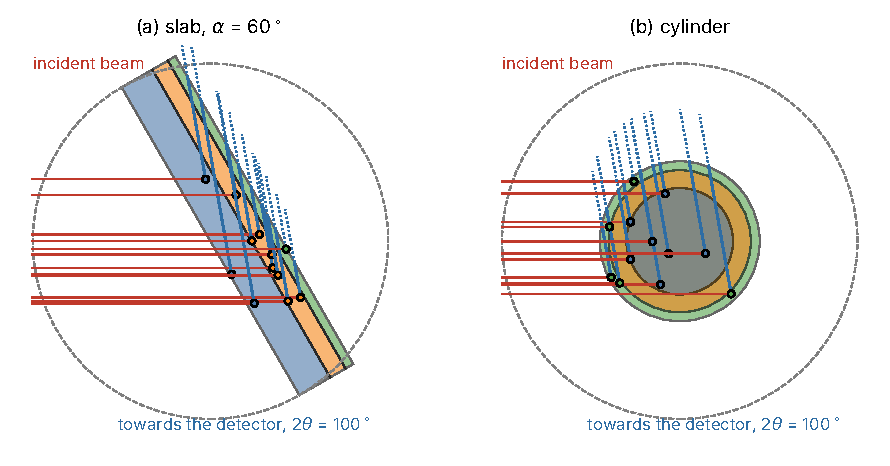
\includegraphics[width=\textwidth]{fig_trajectories}
  \caption{Examples of trajectories. Red: incident particles. Dots: interaction points, coloured by layer.
  Blue: path from the interaction point to the exit of the sample towards the detector ($\twotheta=100^\circ$); the dotted
  continuation only shows the direction. (a)~Slab with $\alpha=60^\circ$. (b)~Cylinder.}
  \label{fig:traj}
\end{figure}
